% !TEX TS-program = pdflatex
% !TEX encoding = UTF-8 Unicode

% Example of the Memoir class, an alternative to the default LaTeX classes such as article and book, with many added features built into the class itself.

%\documentclass[12pt,a4paper]{memoir} % for a long document
\documentclass[12pt,a4paper,article]{memoir} % for a short document

\usepackage[utf8]{inputenc} % set input encoding to utf8

% Don't forget to read the Memoir manual: memman.pdf

%%% Examples of Memoir customization
%%% enable, disable or adjust these as desiredUntitled

%%% PAGE DIMENSIONS
% Set up the paper to be as close as possible to both A4 & letter:
\settrimmedsize{11in}{210mm}{*} % letter = 11in tall; a4 = 210mm wide
\setlength{\trimtop}{0pt}
\setlength{\trimedge}{\stockwidth}
\addtolength{\trimedge}{-\paperwidth}
\settypeblocksize{*}{\lxvchars}{1.618} % we want to the text block to have golden proportionals
\setulmargins{50pt}{*}{*} % 50pt upper margins
\setlrmargins{*}{*}{1.618} % golden ratio again for left/right margins
\setheaderspaces{*}{*}{1.618}
\checkandfixthelayout 
% This is from memman.pdf

%%% \maketitle CUSTOMISATION
% For more than trivial changes, you may as well do it yourself in a titlepage environment
\pretitle{\begin{center}\sffamily\huge\MakeUppercase}
\posttitle{\par\end{center}\vskip 0.5em}

%%% ToC (table of contents) APPEARANCE
\maxtocdepth{subsection} % include subsections
\renewcommand{\cftchapterpagefont}{}
\renewcommand{\cftchapterfont}{}     % no bold!

%%% HEADERS & FOOTERS
\pagestyle{ruled} % try also: empty , plain , headings , ruled , Ruled , companion

%%% CHAPTERS
\chapterstyle{hangnum} % try also: default , section , hangnum , companion , article, demo

\renewcommand{\chaptitlefont}{\Huge\sffamily\raggedright} % set sans serif chapter title font
\renewcommand{\chapnumfont}{\Huge\sffamily\raggedright} % set sans serif chapter number font

%%% SECTIONS
\hangsecnum % hang the section numbers into the margin to match \chapterstyle{hangnum}
\maxsecnumdepth{subsection} % number subsections

\setsecheadstyle{\Large\sffamily\raggedright} % set sans serif section font
\setsubsecheadstyle{\large\sffamily\raggedright} % set sans serif subsection font

%% END Memoir customization

% SEE INCLUDED .tex FILE FOR TITLE CUSTOMIZATION
% title customization/design/whatever
\title{Isn't autumn lovely?}
\author{MC Frontalot}
\date{} % Delete this line to display the current date


%%% BEGIN DOCUMENT
\begin{document}
% Titlepage
% Titlepage
\begin{titlepage}
\begin{tikzpicture}[remember picture,overlay]
    \node[yshift=-10cm, xshift=0.01cm] at (current page.north west)
      {\begin{tikzpicture}[remember picture, overlay]
           \draw[top color=red, bottom color=DarkRed] (0,0) rectangle
                (\paperwidth-0.02cm,10cm);
           \node[anchor=west, yshift=3cm, xshift=2cm, scale=0.2cm]
                {\color{white} \thetitle};
           \node[anchor=west, yshift=0.5cm, xshift=17cm, scale=1.5]
                {\color{white} \thedate};
           \node[anchor=west, yshift=-5cm, xshift=2.7cm, align=left]
                {\color{black} \theauthor};
           \node[yshift=-14.5cm, xshift=11cm, align=center]
                {\color{black}\large Eksperter i Team};
           \node[yshift=-15cm, xshift=11cm, align=center]
                {\color{black}\large Norges Teknisk-Naturvitenskapelige Universitet};
       \end{tikzpicture}
      };
   \end{tikzpicture}
\end{titlepage}

% Chapter 0 - Abstract
\chapter*{Sammendrag}
%\section{Sammendrag}
Eksperter i Team er et fag som skal gi masterstudenter erfaring med og innsikt i prosjektarbeid.
Denne rapporten beskriver hvordan gruppedynamikken vår har utviklet seg under prosjektet i Eksperter i Team.
Vi skal se hvordan gruppens bevissthet i forhold til sin egen rolle i gruppa endrer seg, og hvordan gruppen behersker å bytte på roller fra dag til dag.
Rapporten viser hvordan vi har reflektert over ting som påvirker samarbeidet, og iverksatt aksjoner for å forbedre det. 
Vi viser hvilke utgangspunkt gruppen hadde før prosjektet startet, og hvor vi endte opp til slutt. 
Gruppen som helhet sitter igjen med en mye større innsikt i en gruppes roller og dynamikk. 
Samtlige har tilegnet seg ``verktøy'' som kan benyttes i fremtidige samarbeidsprosjekter.
\vspace{\secspace}

Første del av samarbeidet var preget av en ``bli-kjent''-fase.
Denne delen var mindre produktiv, og det var her gruppen skulle forme sine mål og normer. 
Etterhvert som gruppen definerte arbeidsoppgavene ble arbeidet mer strukturert og effektiviteten økte. 
Samtidig som gruppens effektivitet økte, økte også samholdet innad i gruppen. 
Det ble gjennomført en rullerende lederstruktur som hjalp alle med å få bedre innsikt i sin egen rolle, samt utfordre seg selv til å prøve noe nytt. 
Dette hadde varierende hell med tanke på effektivitet, men økte læringsutbyttet betraktelig. 
\vspace{\secspace}

Kommunikasjonen i gruppa var i begynnelsen skjevt fordelt. 
Noen snakket mye, mens andre holdt seg mer i bakgrunnen. 
Dette ble mye bedre etter at gruppen hadde en åpen diskusjon om kommunikasjonsmønstret, og dermed ble alle mer bevisst på hvordan de selv ble oppfattet av de andre. 
Gruppen har opparbeidet seg et positivt kommunikasjonsklima som oppfordrer til åpne diskusjoner og lav terskel for å ta opp ting. 

\vfill
\begin{center}
Vi ønsker å takke landsbyleder Sven Fjeldaas for teknisk veiledning, og fasilitatorene Henrik André Pedersen og Hanne Schøld Sæterdal for hjelp med prosess-delen.
\end{center}


% Make table of contents
\tableofcontents

% Chapter 1 - Introduction
\chapter{Innledning}
THIS IS A REFERENCE \cite{levin}
\lipsum[1-4]


\newpage

% Chapter 2 - Background
\chapter{Bakgrunn}
For å kunne dokumentere utviklingen til gruppen, samt utviklingen til den enkelte, er det viktig å vite utgangspunktet.


             % Introduction to chapter
\section{Hva er en gruppe}
Til å begynne med må et team/arbeidsgruppe defineres. 
Det finnes mange definisjoner på dette, men gruppen valgte å rette seg etter Katzenbach og Smith som lyder som følger: 

\begin{center}
\textit{Et team defineres som flere personer som arbeider sammen for å oppnå et felles mål. \newline
Medlemmene må være avhengige av hverandre på en eller annen måte.}
\newline 
\citep{katzenbach}
\end{center}

En gruppe settes med andre ord ofte sammen for å oppnå et mål som er vanskelig/umulig å oppnå alene. 
Det er ikke slik at det alltid er fordelaktig å jobbe i gruppe, men komplekse flerfaglige/uoversiktlige oppgaver blir gjerne enklere å løse i grupper.
Gruppearbeid kan også gi løsninger preget av en større grav av nyskapning og kreativitet. 
Generelt er den største motivasjonen for å arbeide i en gruppe at større prosjekter har en veldig stor grad av tverrfaglighet. 
Dette er noe som kommer godt frem i arbeidslivet også \citep{levin}. 
En gruppe bør ikke bestå av mer enn 10 personer, men 5-6 regnes av Katzenbach som den optimale størrelsen.
                   % What is a team?
\section{Gruppens forventninger til EiT}

%% Anders %%
\begin{table}[H]
\begin{tabular}{l l}
        Navn: & Anders Strand \\
        Alder: & 24 år \\ 
        Linje: & Teknisk Kybernetikk \\
        Styrke: & Tar initiativ \\
        Svakhet: & Dominerende
    \end{tabular}
\end{table}

Mine første tanker om EiT kom hovedsakelig fra venner og kjente som har hatt faget før.
De hadde hatt både gode og dårlige opplevelser, og jeg fikk tips til hvordan jeg kunne få mest mulig ut av faget. 
Jeg brukte denne informasjonen da jeg søkte landsby, og fikk mulighet til å prege prosjektet i stor grad. 
Jeg fikk derfor ha et prosjekt jeg synes var spennende og lærerikt.
Prosessdelen av faget var jeg spent på, men hadde ikke den negative innstillingen flere hadde til å begynne med. 
Jeg var åpen for å lære mye om samarbeid, og lære meg selv bedre å kjenne. 
Jeg kan relatere disse emnene opp mot frivillige verv jeg har på fritiden, og også faget Ledelse i Praksis som jeg tar parallelt med EiT.

\bigskip

%% Petter %%
\begin{table}[H]
    \begin{tabular}{l l}
        Navn: & Petter S. Storvik \\
        Alder: & 22 år \\ 
        Linje: & Elektronikk \\
        Styrke: & Målrettet \\
        Svakhet: & Noe begrenset relevante kunnskaper
    \end{tabular}
\end{table}

I og med at studenter som har hatt EiT kun har ytret seg negativt om faget, var jeg tildels negativt innstilt i begynnelsen. 
Landsbyens tema var mitt førstevalg, og skulle være interessant nok til å kompensere for prosessdelen. 
Til tross for min negative holdning var jeg innstilt på å få mest mulig ut av EiT.
Derfor valgte jeg å være åpen mot prosessdelen og prøve å engasjere meg mest mulig i denne delen av faget. 
I og med at jeg ikke kjente noen der fra før, var jeg spent på å bli kjent med gruppen og begynne med det tekniske prosjektet. 


\bigskip

%% Odd %%
\begin{table}[H]
\begin{tabular}{l l}
        Navn: & Odd Magnus Trondrud \\
        Alder: & 22 år \\ 
        Linje: & Datateknikk \\
        Styrke: & Lur type \\
        Svakhet: & Ekstremprokrastinerer
    \end{tabular}
\end{table}

Jeg regnet med å måtte bruke semesterets onsdager på EiT.
Jeg visste ikke hva tiden faktisk ville gå med til, men jeg håpet at det ikke ville være spesielt krevende.
Gjennom frivillige verv og dataspill hadde jeg allerede erfart det å måtte jobbe med og bli kjent med fremmede mennesker.
De holdningene til EiT jeg hadde observert hos folk som hadde tatt faget tidligere var i hovedsak negative.
Kombinert med mine egne erfaringer fra eget studieløp og -assistentstillinger ved NTNU, samt intervjuprosessen for EiT-læringsassistentene, ga dette meg ingen grunner til å være positivt innstilt til faget.
Heldigvis bruker jeg bevisst så lite tid som mulig på å være negativ til obligatoriske aktiviteter da jeg føler det har en ufordelaktig påvirkning på livskvaliteten min.
Holdningen min kan oppsummeres som ``ubegeistret og nøytral''.


\bigskip

%% Ole %%
\begin{table}[H]
\begin{tabular}{l l}
        Navn: & Ole S. Bauck \\
        Alder: & 23 år \\ 
        Linje: & Teknisk Kybernetikk \\
        Styrke: & Engasjert\\
        Svakhet: & Komme tidsnok
    \end{tabular}
\end{table}

Mine forventninger til EiT var at dette kom til å bli et spennende prosjekt, til tross for all neqative kommentarer jeg har hørt om faget. 
Landsbyens tema var ikke mitt førstevalg, men siden vi det var noen personer i gruppen som kjente hverandre og hadde samme interesseområde, så tenkte jeg at det kom til å bli interessant allikevel.

Det eneste jeg var litt spent på var hvordan prossessdelen kom til å være, men jeg var bestemt på å komme med en åpen innstilling slik at jeg kunne lære mest mulig av samarbeidet.
\bigskip

%% Emil %%
\begin{table}[H]
\begin{tabular}{l l}
        Navn: & Emil Taylor Bye \\
        Alder: & 2x år \\ 
        Linje: & Teknisk Kybernetikk \\
        Styrke: & \\
        Svakhet: & 
    \end{tabular}
\end{table}

\bigskip
           % Our expectations to EiT
\section{Gruppens personligheter}
En gruppe består av flere enkeltindivider. 
Personligheten til alle i gruppen virker inn på hvordan gruppemedlemmene forholder seg til hverandre. 
Det kan være viktig å kartlegge hvilke personligheter som er i gruppen, slik at det blir lettere å forstå hvorfor gruppen utvikler seg som den gjør.

\subsection{Meyers-Briggs personlighetsindikator}
Meyers-Briggs er bassert på teorier av Carl Gustaf Jung (1921).
Måleter å klassifisere de psykologiske forsjellene mellom mersoner.
Bokstavene i fet skrift vil gi en person en beskrivelse på fire bokstaver, det vil si 16 mulige personlighetstyper.
Denne beskrivelsen vil da gjenpseile person best mulig, og kan derfor brukes til å beskrive gruppemedlemmer og deres forsjeller.
\vspace{\secspace}

\begin{table}[H]
    \centering
    \begin{tabular}{| l | l c r |}
        \hline
        \textbf{Holdning} & Utadvent(\textbf{E}xtraversion) & $\leftrightarrow$ & Innadvendt(\textbf{I}ntrovert) \\ \hline
        \textbf{Funksjon} & Sansing(\textbf{S}ensing) & $\leftrightarrow$ & Intuisjon(i\textbf{N}tuition) \\ \hline
        \textbf{Funksjon} & Tenking(\textbf{T}hinking) & $\leftrightarrow$ & Følelse(\textbf{F}eeling) \\ \hline
        \textbf{Livsstil} & Vurdering(\textbf{J}udging) & $\leftrightarrow$ & Oppfattelse(\textbf{P}ercieving) \\
        \hline
    \end{tabular}
    \label{tab:meyersbriggs}
    \caption{Meyers-Briggs akser}
\end{table}

Tabell~\ref{tab:meyersbriggs} viser hvilke forskjellige akser som Meyers-Briggs legger vekt på, samt hvilke bokstaver som benyttes for de forskjellige resultatene.
\textbf{Holdning} er ganske selvforklarende, og forteller om en person er utadvent eller innadvent. 
\textbf{Funksjon} deles i to, Sansing-Intuisjon og Tenking-Følelse. 
Sansing-Intuisjon går på hvordan man tolker og oppfatter ny informasjon. 
En person med preferanse for sansing vil stole på klar informasjon, mens intuisjon gjerne har bedre forståelse av abstrakte begreper. 
Tenking-Følelse dreier seg om å ta beslutninger. 
Tenking beskriver en person som tenker over beslutningen logisk og konsistent. 
En person som beskrives av følelser vil sette seg inn i situasjonen og identifisere seg med de involverte parter.
\textbf{Livsstil} beskriver hvordan en person møter verden. 
Vurdering vil da si at personen vurderer det som skjer mer enn å bare oppfatte det. 
Med dette menes at de tenker over hendelser og de ulike inntrykkene. 
En av svakheten til Meyers-Briggs er at hvordan de enkelte personene definerer de ulike begrepene vil variere ut fra hvilken personlighetstype de har. 
Derfor er ikke aksene så uavhengige som de egentlig skulle vært. 


\subsection{Gruppemedlemmene} \label{chap:meyersgroupmembers}
For å avgjøre hvilke personligheter gruppa bestod av brukte vi et gratis verktøy på internett\citep{mbtest}. 
Dette verktøyet bestemmer din personlighet på grunnlag av 70 spørsmål. 
Grunnen til at vi brukte dette verktøyet fremfor å klassifisere oss seg, var at et slikt verktøy resulterer gjerne i bedre resultater. 
Kvaliteten på akkurat denne testen vet vi forøvrig ikke noe om. 
Alle tok denne testen hver for seg og reulstatet ble drøftet. 

\begin{table}[H]
    \centering
    \begin{tabular}{| l | l | l l l l |}
        \hline
        \textbf{Anders} & ENTJ & \textbf{E}xtravert(33\%) & i\textbf{N}tuitive(50\%) & \textbf{T}hinking(25\%) & \textbf{J}udging(67\%)  \\ \hline
        \textbf{Emil} & INTJ & \textbf{I}ntrovert(56\%) & i\textbf{N}tuitive(12\%) & \textbf{T}hinking(1\%) & \textbf{J}udging(11\%)  \\ \hline
        \textbf{Petter} & ISTJ & \textbf{I}ntrovert(30\%) & \textbf{S}ensing(40\%) & \textbf{T}hinking(75\%) & \textbf{J}udging(67\%)  \\ \hline
        \textbf{Odd} & ENTJ & \textbf{E}xtravert(11\%) & i\textbf{N}tuitive(38\%) & \textbf{T}hinking(25\%) & \textbf{J}udging(67\%) \\ \hline
        \textbf{Ole}  & ISTJ & \textbf{I}ntrovert(33\%) & \textbf{S}ensing(01\%) & \textbf{T}hinking(75\%) & \textbf{J}udging(01\%)  \\
        \hline
    \end{tabular}
    \label{tab:meyersmemb}
    \caption{Meyers-Briggs resultat}
\end{table}

Beskrivelsene av de forskjellige personlighetstypene er hentet fra \textit{Meyers-Briggs foundation}\citep{mbtypes}.
\vspace{\secspace}

\textbf{ENTJ} (the commander) tar gjerne avgjørelser og lederskap enkelt. 
De ser raskt ulogiske og ineffektive prosedyrer og liker langsiktig planlegging og målsetting. 
Vanligvis godt belest og kunnskapsrik. 
Liker å utvide kunnskapene sine og lære ting videre til andre. 
\vspace{\secspace}

\textbf{INTJ} (the mastermind) er ofte innsiktsfull om andre. 
De søker mening i og sammenhenger mellom forskjellige ideer og forhold, og er pliktoppfyllende og forpliktet til sine faste verdier. 
Ofte organisert og prøver å finne ut hvordan man kan tjene det felles beste. 

\textbf{ISTJ} (the inspector) er ofte stille og satser mye på pålitelighet og grundighet. 
De innehar ofte praktiske ferdigheter, og er ansvarlige og realistiske. 
Arbeider jevnt og trutt med det som skal gjøres, til tross for distraksjoner. 
Setter ofte pris på tradisjoner og liker at ting er velorganiserte og ryddige. 

\subsection{Sammensetningen}
Det kommer godt frem av Meyers-Briggs, og forsåvidt presentasjonen av gruppemedlemmene, at gruppen har i stor grad lik faglig sammensetning.
Ofte brukes to begreper om dette, de blir ifølge videoforelesninger\citep{video} i EiT: 
\vspace{\secspace}

\textbf{Homogen gruppe} vil si at gruppemedlemmene har liten faglig spredning. 
En slik gruppe vil være mest effektiv når prosjektet har begrenset omfang og er lite flerfaglig. 
Fordelen med en slik gruppe er at gruppemedlemmene kommer ofte godt overens og har derfor gjerne mindre sosiale utfordringer. 
Det er også noen bakdeler med en homogen gruppe. 
Homogene grupper har en tendens til å unngå risikoer, og dermed går glipp av muligheter. 
De har også problemer med å tilpasse seg dynamiske situasjoner.
\vspace{\secspace}

\textbf{Heterogen gruppe} er det motsatte av en homogen gruppe. 
Dette er en gruppe preget faglig spredning og er ofte bedre til å ta viktige beslutninger samt tenke nytt og kreativt enn homogene grupper. 
Til tross for dette er det ikke gitt at en faglig spredt gruppe resulterer i suksess. 
Ofte kan heterogene grupper ha større utfordringer når det kommer til intern kommunikasjon eller problemer med at medlemmer blir defensive og derfor mindre produktive. 
\vspace{\secspace}

Da gruppen er et godt eksempel på en homogen gruppe kan noen av utfordringene over bli reelle.
% TODO skriv en setning eller to mer på avslutningen av dette avsnittet           % Meyers Briggs - test
Et verktøy for å visualisere hvordan gruppens medlemmer står i forhold til hverandre kalles samarbeidsindikatorer. 
Verktøyet er utarbeidet av Are Holden i samarbeid med EiT-staben. 
Dette var et tilbud alle gruppene i landsbyen fikk og testen ble gjennomført av fasilitatorene. 
Undersøkelsen ble gjennomført ved at vi svarte på en rekke spørsmål anonymt, disse svarene ble så grunnlaget for en graf som illustrerer hvordan gruppen ligger an.
Denne grafen belyser områder som gruppen har små, middels eller store utfordringer på. 
For å oppdage eventuell fremgang ble denne testen gjort to ganger iløpet av EiT-kurset. En gang helt i begynnelsen (2. landsbydag) og en gang mot slutten av prosjektet (10. landsbydag). 

\subsection{2. landsbydag}
På grunn av at den første testen ble tatt i en tidlig fase av gruppearbeidet, gir den et godt inntrykk av gruppens initielle situasjon. 
På grafen er det to linjer, en heltrukken rød og en en stiplet rød. 
Disse linjene markerer grensene på hvor ting blir regnet som store problemer og små problemer. 
\begin{figure}[H]
    \centering
    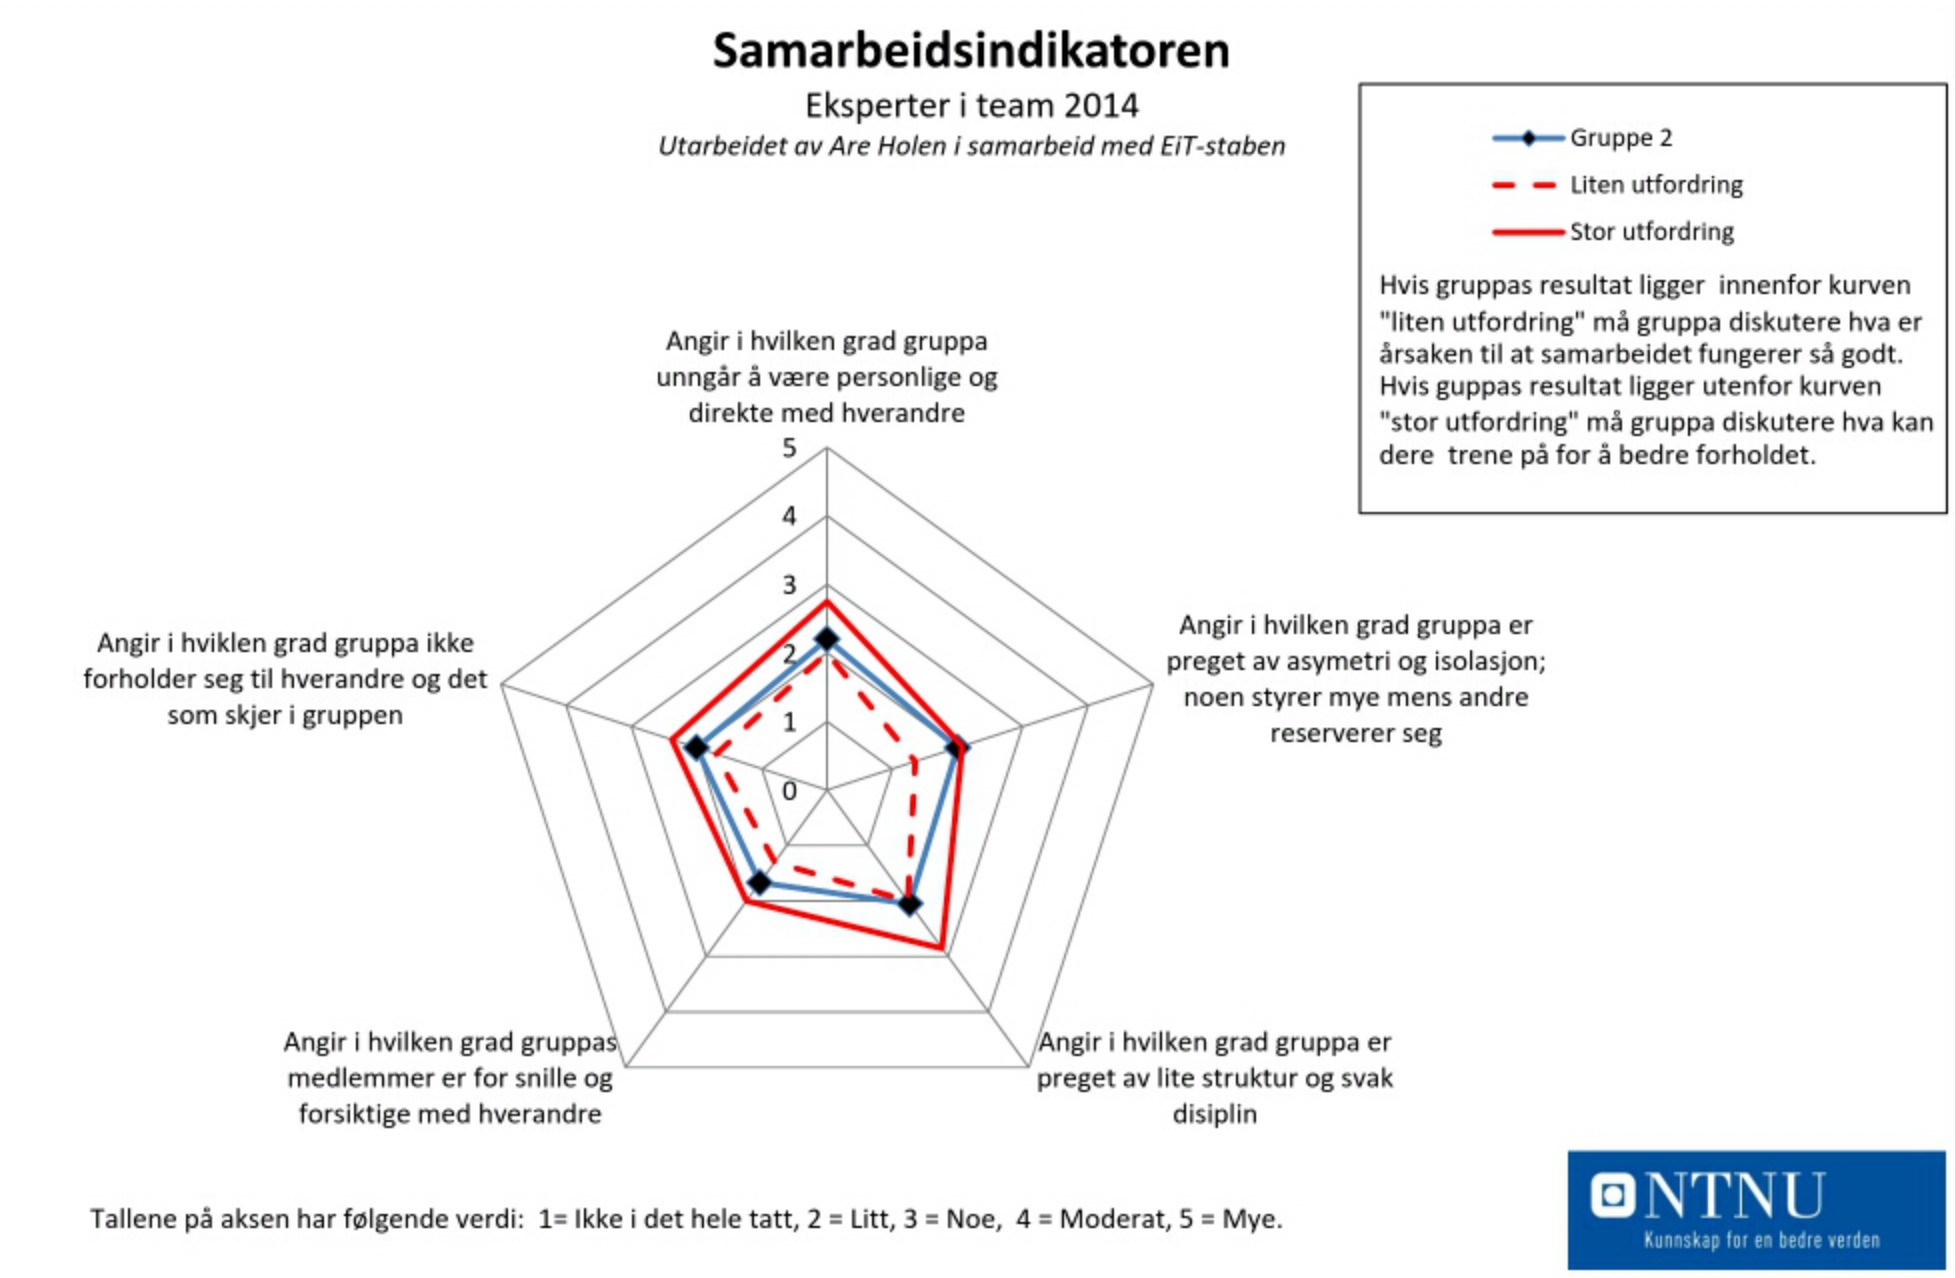
\includegraphics[width=0.7\textwidth]{images/samarbeidsindikator1.jpeg} 
    \caption{Samarbeidsindikatorer 2. landsbydag}
    \label{fig:sam1}
\end{figure}

\noindent \textbf{I hvilken grad gruppen unngår å være personlig:} 2.2.
\newline
\noindent Her hadde vi en moderat utfordring, noe som faller naturlig ettersom vi var en nydannet gruppe.
 At vi selv er bevisste på dette er et godt tegn, noe som gjenspeiler vårt fokus på dette området i videre prosessjobbing.
\vspace{\secspace}

\noindent \textbf{I hvilken grad gruppen er preget av asymmetri og isolasjon:} 2.
\newline
\noindent Gruppen hadde de første dagene to medlemmer som var mest dominerende; Odd og Anders.
De tre resterende medlemmene hadde til da tatt en passiv posisjon og var ikke like aktive i felles aktiviteter. 
Under diskusjon av testens resultat, kom vi frem til at dette punktet er noe vi bør jobbe mye med. Vi definerte en aksjon, som var å rullere på å ha lederrollen i gruppa. 
Isolasjon er noe vi følte vi hadde lite av, så det passet dårlig at disse punktene var slått sammen. Vi har hele tiden lagt vekt på at alle i gruppen skal bli hørt, og tas seriøst. 

\vspace{\secspace}

\noindent \textbf{Hvilken grad gruppen er preget av lite struktur:} 1.
\newline
\noindent Som nevnt i punktet over tok noen tak og skapte rammer for arbeidet tidlig i prosessen. Dette gjorde at vi fra begynnelsen jobbet strukturert mot et felles mål. Vi var altså tidlig i prosessen preget av god struktur, og det viste seg i ettertid at grunnarbeidet gjort i den tidlige fasen la grunnlag for en god oppdeling av arbeidet. 
\vspace{\secspace}

\noindent \textbf{Hvilken grad gruppen er for snille med hverandre:} 1.8.
\newline
\noindent Vi kjente hverandre ikke så godt på dette tidspunktet, så dette kan virke naturlig. Vi satte likevel mål om å utvikle en trygghet og respekt for hverandre slik at det blir lettere å være ærlig og konstruktiv.
\vspace{\secspace}

\noindent \textbf{Hvilken grad gruppen ikke forholder seg til hverandre:} 1.
\newline
\noindent Vi hadde fra starten en god tone i gruppa, og ingen meldte seg ut eller ble fryst ut. Indikatoren viser her at dette ikke var et problem i noen særlig grad.

\subsection{10. landsbydag}
\begin{figure}[H]
    \centering
    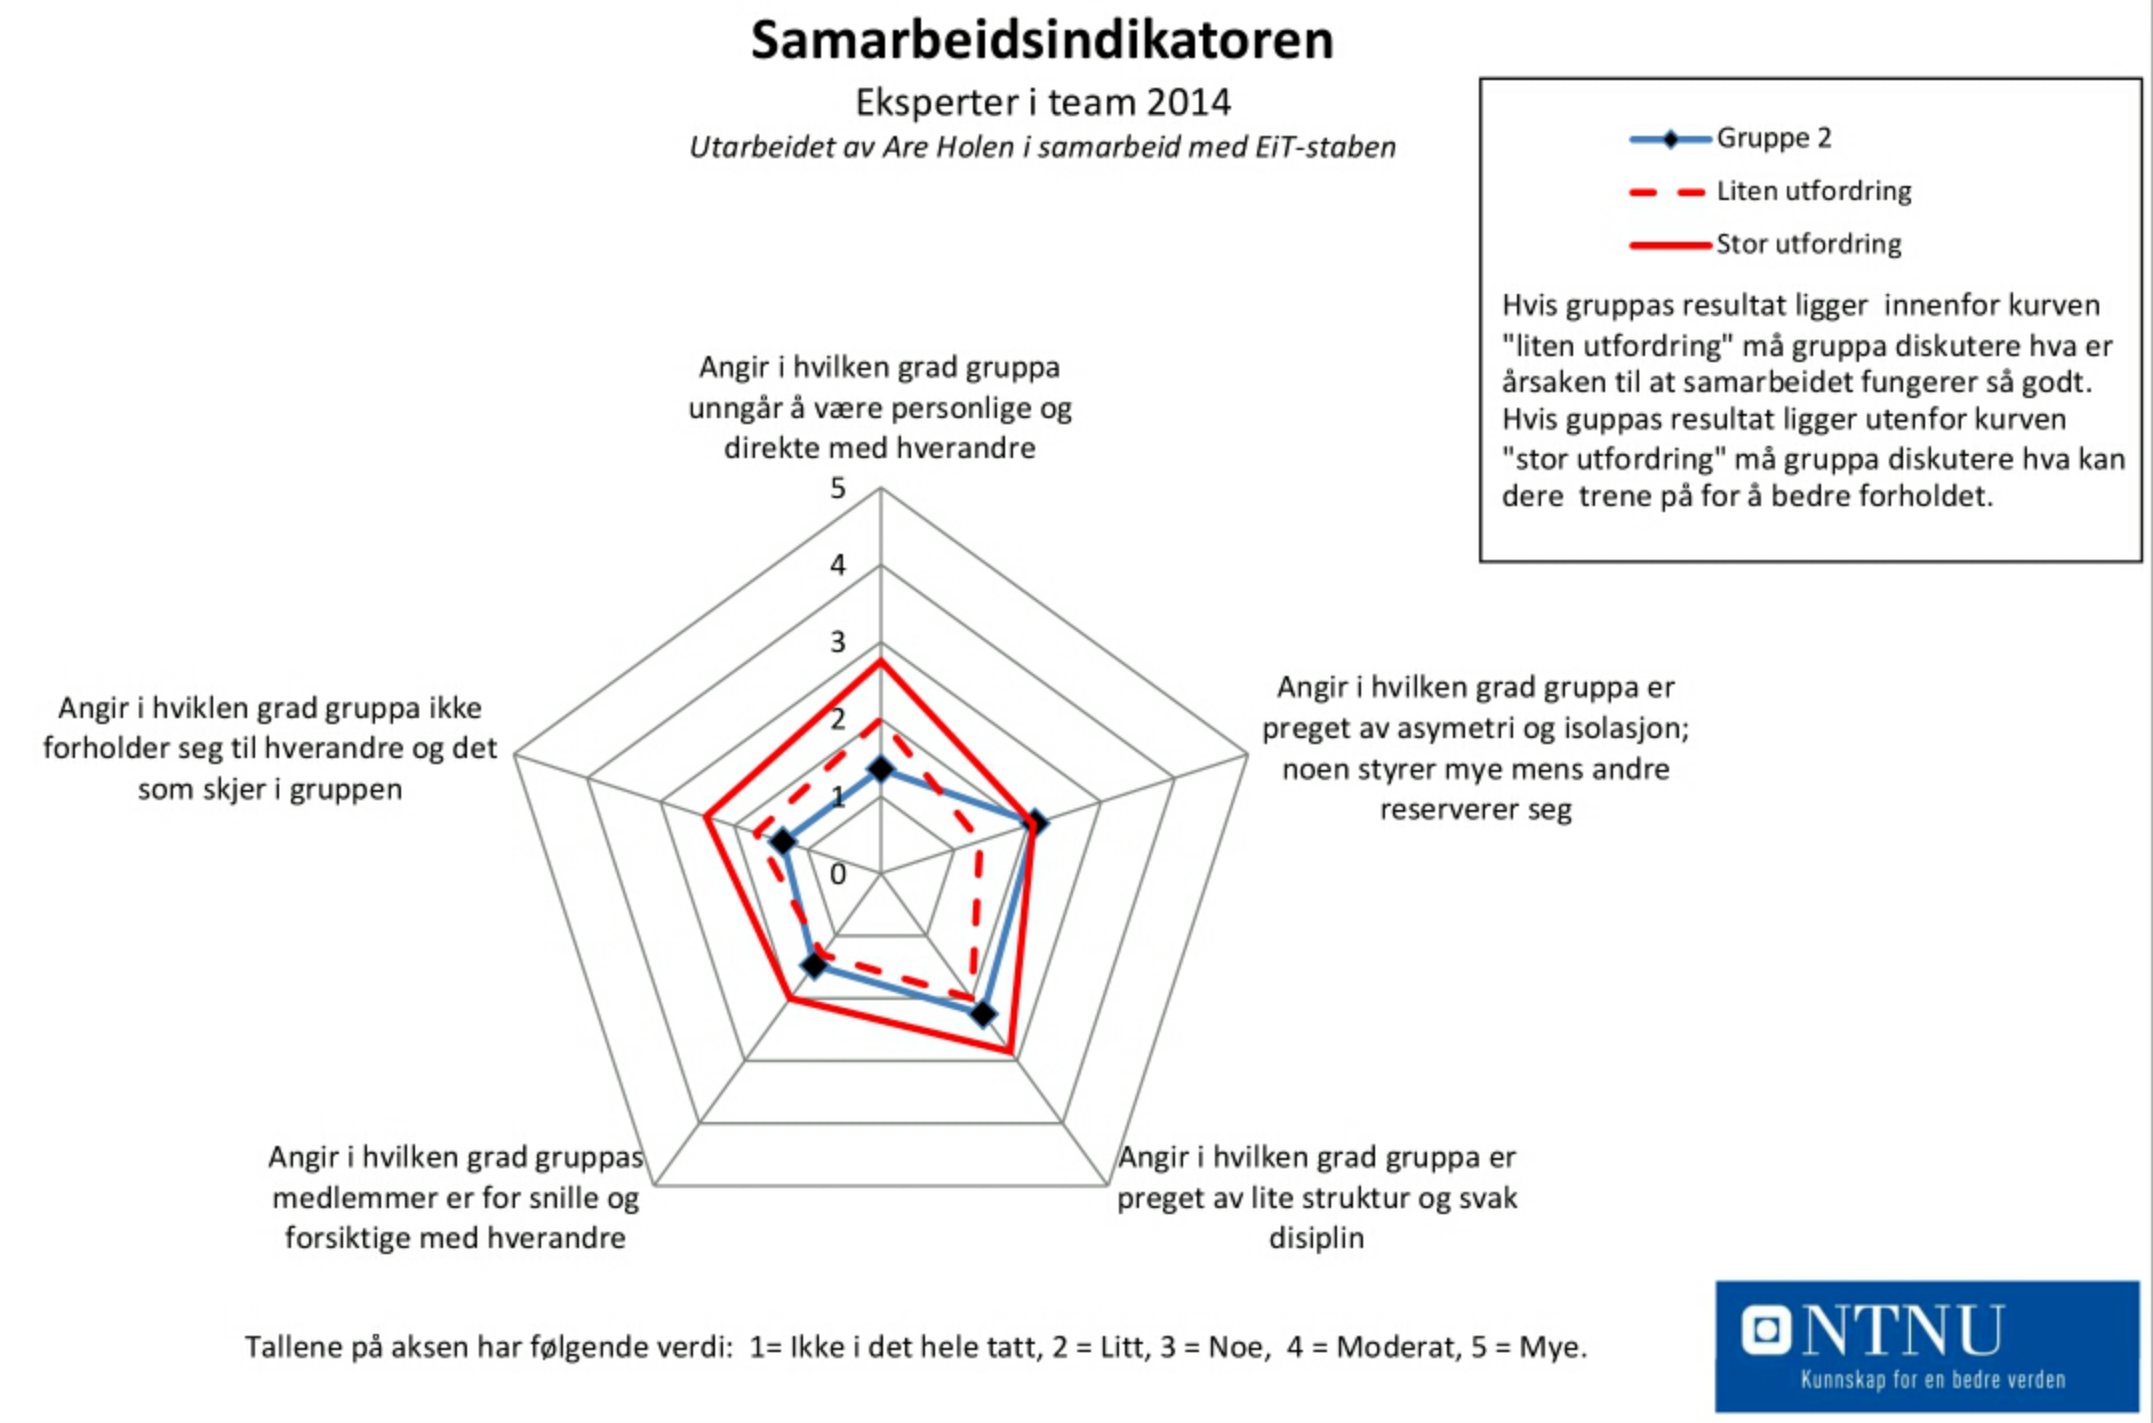
\includegraphics[width=0.7\textwidth]{images/sam2.png} 
    \caption{Samarbeidsindikatorer 10. landsbydag}
    \label{fig:sam2}
\end{figure}

\noindent \textbf{I hvilken grad gruppen unngår å være personlig:} 1.5.
\newline
\noindent Her ser vi en nedgang i forhold til første undersøkelse. Dette gjenspeiler hvordan vi etter hvert har blitt flinkere til å gi ærlige tilbakemeldinger. Hver arbeidsdag har vi brukt 1,5 timer på slutten av dagen til å reflektere over samarbeidet. 
Dette har skapt en arena hvor listen for å ta opp ting er lav, og vi har vært veldig åpne for konstruktiv kritikk.
\vspace{\secspace}

\noindent \textbf{I hvilken grad gruppen er preget av asymmetri og isolasjon:} 2.
\newline
\noindent På dette punktet har vi fortsatt en ganske høy verdi. Da vi reflekterte over dette resultatet var det ingen som kjente seg igjen i dette. Når det er sagt, så er forsatt aktivitetsnivået i gruppa varierende.
Vi er nå trygge på at de som ønsker å si noe tar ordet, og blir hørt. Hvis man er stille betyr det nå at man er enig, eller ikke har noe spesielt å komme med. I tidligere faser var det kanskje andre grunner til at noen ikke tok ordet. 

\vspace{\secspace}

\noindent \textbf{Hvilken grad gruppen er preget av lite struktur:} 2.2.
\newline
\noindent Vår rullering av lederrollen førte til mange nyttige refleksjoner og erfaringer. 
Samtidig førte det til lite struktur enkelte dager, ettersom graden av lederskap varierte stort fra person til person. For noen var det lett å glemme rollen som leder utover dagen, og falt tilbake i gamle vaner med å trekke seg tilbake. 
Vi opplevde også at gruppen etter hvert begynte å bli litt lei prosjektet, og hadde lettere for å komme med avsporinger.
Prosjektet hadde en god fremgang, og vi så at vi kom til å blir ferdig med det aller meste vi hadde planlagt.
Dette førte til at mye av arbeidslysten minsket.
\vspace{\secspace}

\noindent \textbf{Hvilken grad gruppen er for snille med hverandre:} 1.5.
\newline
\noindent Vi har også her en liten nedgang fra første test. Det at vi ikke enda er fullstendig ærlige og direkte kan forklares av flere ting. 
Rent teknisk har prosjektet vårt gått veldig bra, og kommunikasjonen og samarbeidet har vært godt hele veien. Problemer ved arbeidsmetoder ble jevnlig reflektert over i felleskap, og påfølgende aksjoner ble satt i gang. Vi har altså ikke hatt noen store problemer eller problempersonligheter som har krevd en hardere tone i gruppen. 
\vspace{\secspace}

\noindent \textbf{Hvilken grad gruppen ikke forholder seg til hverandre:} 1.5.
\newline
\noindent Etter hvert som planleggingen var ferdig og den tekniske implementasjonen ble satt i gang, begynte vi å arbeide mer selvstendig. Dette førte til mindre kommunikasjon i en gruppe som helhet, men introduserte heller tettere samarbeid mellom enkelte grupperinger. Vi ser på dette som naturlig i den fasen av arbeidet.
I starten delte vi oss opp på to forskjellige bord for å få plass til alt utstyret vi jobbet med. Etter et par dager hadde vi en grundig diskusjon på om dette var riktig, og kom frem til at vi alle burde sitte rundt samme bord selv om vi jobbet selvstendig, 
Vi reflekterte senere over hvordan dette innvirket på arbeidet vårt. 
Det ble lettere å spørre om små ting man lurte på, vi fikk alle en større innsikt i hva hverandre holdt på med. 
Det var spesielt det at vi ikke satt med ryggen til hverandre, men heller rundt et større bord som var utslagsgivende. 
  % Cooperation indicators 
\section{Utarbeidelse av samarbeidsavtale}
En samarbeidsavtale mellom gruppemedlemmene blir sett på som en viktig og nødvendig del av et effektivt gruppearbeid. 
MRPI-modellen, som er basert på arbeid av David Kolb (1986) er en god mal for en samarbeidsavtale. 
Denne sier at en avtale bør bestå av:
\begin{itemize}
  \item \textbf{M}ål
  \item \textbf{R}oller
  \item \textbf{P}rosedyrer
  \item \textbf{I}interpersonlige forhold
\end{itemize}
Med andre bør avtalen bør inneholde svar på hvilke mål gruppen har, de ulike rollene i gruppen, hvordan beslutninger skal tas, hvordan gruppemedlemmene skal forholde seg til hverandre og øvrige formaliteter \citep{levin}.

\subsection*{Første utgave}
Den første utgaven av avtalen ble utarbeidet i starten av gruppearbeidet. 
Avtalens utforming var bassert på en mal som ble utdelt i landsbyen. 
Denne malen fortalte hvilke kategorier som kunne være lure å ha med, samt noen viktige punkter innen disse kategoriene. 
På grunn av at gruppens medlemmer ikke kjente hverandres måter og jobbe på var gruppen klar over at samarbeidsavtalen måtte revideres senere ut i gruppearbeidet. 
\vspace{\secspace}

Vi valgte å bruke følgende kategorier:
\begin{itemize}
    \item \textbf{Leveranse} - Omfatter arbeidmenge, metode, mål i faget, o.l.
    \item \textbf{Trivsel} - Det som går på det sosiale i gruppen. 
    \item \textbf{Læring} - Dette punktet følte gruppen var nødvendig for å maksimere læringsutbyttet i EiT. 
    \item \textbf{Annet} - Her står det som ikke passser inn i de andre kategoriene. Er også nevnt hvordan de ulike rollene i gruppen fordeles. 
\end{itemize}
Samarbeidsavtalen ligger som Vedlegg 1. 

\subsection*{Andre utgave}
Midt i prosjektoppgaven ble samarbeidsavtalen revidert. 
Dette ble gjort i forbindelse med et initiativ fra fasilitatorene, og ble tatt felles for hele landsbyen. 
Gruppen var enige om at en systematisk gjennomgang av hele samarbeidsavtalen der vi diskuterte hva som hadde fungert bra og hva som kunne vært bedre. 
Den reviderte samarbeidsavtalen ligger som Vedlegg 2. 
\vspace{\secspace}

\noindent Det som ble forandret eller lagt til var: 
\begin{enumerate}
  \item Følge dagsplanen: Dagsplanen er et eget dokument som sier hvilke faste aktiviteter som skal gjøres og når. Leder har ansvar for at disse følges. 
  \item Alle aksjoner som bestemmes skal settes inn i eget aksjonsdokument. Dette dokumentet er for å lettere holde styr på det som blir vedtatt.
  \item Lederrollen skal rullere. Slik vil alle få best mulig læringsutbytte av EiT. 
\end{enumerate}

Den første samarbeidsavtalen var med andre ord ganske bra, derfor ble ikke så mye forandret/lagt til. 
Dette er også en indikator på at gruppen var flink til å følge det som ble satt i avtalen. 
        % How we formed the group agreement
\newpage

% Chapter 3 - Group reflections
\chapter{Gruppens utvikling}

For å beskrive gruppens utvikling gjennom hele prosjektet brukes modellene som ble beskrevet i teori-delen.
Gruppen mener at Halvtidsmodellen blir for liten for å beskrive utviklingen.
                       % Introduction to chapter
\section{SITRA-modellen}
SITRA modellen er en modell som tar sikte på å gjøre skillet mellom situasjoner, observasjoner og aksjoner tydeligere.
Hovedelementene er:

\begin{enumerate}
  \item \textbf{Situasjon} - Den situasjonen som observeres.
  \item \textbf{Teori} - Relevant teori som kan knyttes til situasjonen.
  \item \textbf{Refleksjon} - Gruppens tanker rundt situasjonen.
  \item \textbf{Aksjon} - Noe som gruppen gjør for å forbedre dette. 
\end{enumerate}

I gruppens tilfelle ble en begrenset versjon av SITRA-modellen brukt. 
Derfor inneholder grupperefleksjonene hovedsaklig de tre punktene, situasjon, refleksjon og, i de tilfellene det trengs, aksjon.
Gruppen har bevisst prøvd å forme gruppeloggen etter SITRA-modellen, slik at det blir enklere å se på gruppens fremgang i ettertid. 
Slik blir det også enklere å knytte inn relevant teori når gruppens utvikling analyseres.                        % Description of SITRA
\section{Faser og effektivitet}
Det har vært gjort utallige forsøk på å beskrive hvordan en gruppe utvikler seg over tid. 
De fleste modellene basserer seg på ulike faser som en typisk gruppe går gjennom. 
Ikke alle grupper går gjennom alle fasene, og det kan være vanskelig å identifisere hvilke fase en gruppe er i.
Til tross for at disse modellen er godt utviklet og forstått er det ingen modell som nøyaktig vil beskrive en gruppeprosess, men de hjelper oss å forstå de ulike forandringene som en gruppe går gjennom. 
Ofte kan en gruppes utvikling beskrives av en kombinasjon av diverse modeller (Levin 2012). 
\vspace{\secspace}

\textit{Halvtidsmodellen}, utviklet av Gersick (1989), tar utgangspunkt i studenter som arbeider med prosjektoppgaver som en del av sitt universitetsstudium.
Ofte blir denne modellen nevnt i forbindelse med prosjektoppgaver i studiet. 
Denne modellen består av to faser, der fase 1 er første halvdelen av prosjektet og fase 2 er andre halvdelen. 
Halvveis i prosjekter er her når studentene oppfatter de er halvveis, ikke nødvendig halvveis med tanke på arbeidsmendge. 
Det som kjennetegner halvtidsmodellen er at effektiviteten, strukturen og målene er betydelig høyere i siste halvdel av prosjektet enn i første.
Gruppen mener denne modellen ble for snever for dette tilfellet, men siden den er mye nevnt i lignende sammenhenger var det logisk å beskrive den her. 
\vspace{\secspace}

En modell som beskriver gruppens utvikling godt er \textit{Forming, norming, storming, performing}, som er en modell utviklet av Tuckman \& Jensen (1977). 
Denne modellene søker å beskrive hvorfor det tar tid før en gruppe blir produktiv. 
\textit{Forming} er den første fasen og handler om å innhente informasjon. 
I denne fasen skal gruppen bli kjent, møtes og forme mål/mandat.
Fase nummer to kalles \textit{storming} og er en følelsesmessig fase. 
Her skal gruppen bli enige om hvordan oppgaven skal løses. 
Etterhvert som de lærer hverandre å kjenne finner de også sin plass/rolle i gruppen. 
Gruppetilhørigheten blir sterkere i fasen \textit{norming}. 
Til nå har gruppen etablert normer og regler som gjelder innad i gruppa. 
Siste fase kalles \textit{performing} og er den effektive fasen der mesteparten av problemstillingen blir løst. 
\vspace{\secspace}

\subsection{Fasene}
Som nevnt over kan ikke hele gruppearbeidet beskrives av de modellene som finnes. 
Utviklingen vil være en kombinasjon av de forskjellige modellene og når fasene starter/stopper vil ofte være ''flytende''.
Det vil si at det ikke nødvendigvis er en ''slutt-til-start''-sammenheng mellom de, men gruppen kan befinne seg i flere faser samtidig. 
Under vil gruppens utvikling bli forklart og forsøkt knyttet opp mot de dominerende modellene som beskriver en typisk utvikling. 
Vi har derfor valgt å kun fokusere på de fasene som skiller seg tydelig fra hverandre.
\vspace{\secspace}

%% Fasene vi gikk gjennom 

%%%%%%%%%%%%%%%%%%%%%%%%%%%%%%%%%%%%%%%%%%%%%%%%%%%%%%%
%% Piler side 1
\begin{figure}
    \begin{tikzpicture}[remember picture, overlay, xshift=1cm, yshift=-15.3cm]
        \foreach \x in {0,-1.5,-3,-4.5}%,-6,-7.5,-9,-10.5,-12,-13.5,-15,-16.5}
            \draw [color=white, fill=LightGray, blur shadow] (0,\x) -- (0.5,\x+0.5) -- (0.5,\x-1) -- (0,\x-1.5) -- (-0.5,\x-1) -- (-0.5,\x+0.5) -- (0,\x);
        \draw [color=white, top color=red, bottom color=DarkRed, blur shadow] (0,0) -- (1,1) -- (1,-2) -- (0,-3) -- (-1,-2) -- (-1,1) -- (0,0);
        \draw (0,-0.5) node[anchor=north, color=white] {\Large \textbf{Fase 1}}; 
    \end{tikzpicture}
\end{figure}
\begin{adjustwidth}{2.5cm}{0cm}

\textbf{\Large Fase 1 - Bli kjent}
I begynnelsen av gruppearbeidet skulle gruppen bli kjent med hverandre, dette markerer begynnelse på første fase.
De fleste modeller har en form for initieringsfase der gruppemedlemmene møtes for første gang og stifter bekjentskap. 
Fasilitatorene kjørte noen \textit{bli-kjent}-øvelser som hjalp til med å raskere lære hverandre å kjenne. 
Denne fasen begynte 1. landsbydag og var preget av lite faglig aktivitet. 
Gruppen diskuterte også hvilke forventninger de hadde til prosessbiten og samarbeidet. 
Det ble også kartlagt hvilke kunnskaper og tanker gruppen hadde om den tekniske delen av prosjektet. 
Det var dette som skulle danne grunnlaget for neste fase. 

Johnson \& Johnson (2013) legger vekt på at for å utvikle et effektivt gruppesamarbeid er det viktig at følgende betingelser er oppfyllt:
\begin{enumerate}
    \item Klare og veldefinerte mål
    \item God toveis kommunikasjon
    \item Lederskap og deltakelse noenlunde likt mellom medlemmene
\end{enumerate} 
Gruppen var flink med god kommunikasjon tidlig i prosjektet, men mål og mer lik deltakelse kom med tiden. 
En forklaring på dette kan være at gruppen ikke fikk snakket så mye med hverandre første dagen, da den gikk bort til mange felles ''bli-kjent''-øvelser. 
\vspace{\secspace}

%%%%%%%%%%%%%%%%%%%%%%%%%%%%%%%%%%%%%%%%%%%%%%%%%%%%%%%
%% Piler side 2
\begin{figure}
    \begin{tikzpicture}[remember picture, overlay, xshift=1cm, yshift=1cm]
        \foreach \x in {0,-1.5,-3,-4.5,-6,-7.5,-9,-10.5,-12,-13.5,-15,-16.5,-18,-19.5}
            \draw [color=white, fill=LightGray, blur shadow] (0,\x) -- (0.5,\x+0.5) -- (0.5,\x-1) -- (0,\x-1.5) -- (-0.5,\x-1) -- (-0.5,\x+0.5) -- (0,\x);
        \draw [color=white, top color=red, bottom color=DarkRed, blur shadow] (0,0-7.5) -- (1,1-7.5) -- (1,-2-7.5) -- (0,-3-7.5) -- (-1,-2-7.5) -- (-1,1-7.5) -- (0,0-7.5);
        \draw (0,-0.5-7.5) node[anchor=north, color=white] {\Large \textbf{Fase 2}};
        \draw [color=white, top color=red, bottom color=DarkRed, blur shadow] (0,0-16.5) -- (1,1-16.5) -- (1,-2-16.5) -- (0,-3-16.5) -- (-1,-2-16.5) -- (-1,1-16.5) -- (0,0-16.5);
        \draw (0,-0.5-16.5) node[anchor=north, color=white] {\Large \textbf{Fase 3}};
    \end{tikzpicture}
\end{figure}

\noindent \textbf{\Large Fase 2 - Brainstorming}
Fase 2 var en fase som begynte før gruppen var kommet ut av fase 1. 
2. landsbydag ble det presentert noen alternative oppgaver som vi kunne velge, dette resulterte i at gruppen var usikker på hvilken oppgave vi ville ha. 
For å lettere kunne ta en avgjørelse ble det bestemt at begge de to alternativene skulle diksuteres og drøftes, slik at det ble enklere å ta en beslutning. 
Denne brainstormingen bestod av åpne diskusjoner der alle kunne si sin mening om alternativene. 
Det var meningen at disse diskusjonene skulle være så åpne som mulig, slik at alle fikk komme med sine meninger og ideer. 
Gruppen bestemte til slutt seg for en av oppgavene basert på det som ble diskutert. 
Samtidig som dette ble gjort, lærte medlemmene hverandre å kjenne. 
De interne reglene som er beskrevet i samarbeidsavtalen ble formet og vi begynte å følge disse. 

De to første fasene ligner veldig på begynnelsen av modellen til Tuckman \& Jensen, \textit{Forming, norming, storming, performing}. 
Denne modellen legger vekt på at prosjektets mål/mandat og gruppens normer/regler formes i begynnelsen av prosjektet. 
Normer kan beskriv som hvordan de andre \textit{forventer} at medlemmene skal oppføre seg (Schwarz 2002). 
At alle var med på å forme problemstillingen etter det de kunne/ville lære mener vi hjalp til med å holde motivasjonen oppe lengre ut i prosjektet. 
\vspace{\secspace}

\noindent \textbf{\Large Fase 3 - ''Somlefasen''}
Etter at problemstillingen var formet var prosjektet preget av en fase der ting tok tid. 
Det var deler av prosjektet som var avhengige av at noen komponeneter fungerte sammen med gitt hardware, og det ble derfor en del knoting før dette fungerte.  
I gruppeloggen fremkommer det at flere var litt misfornøyde med framgangen i denne fasen. 
Dette var heller ikke en fase alle gruppemedlemmene var med på. 
Oppdelingen av prosjektet gjorde at de som ikke jobbet med denne delen kunne jobbe uavhengig av somlingen. 
Slik oppretholdte gruppen en bedre fremgang enn den ellers ville klart. 

Dette er ikke en fase man vanligvis ser så tidlig i prosjektet, men kan sammenlinges med stagnasjonsfasen i \textit{Åtte faser}-modellen av Rosen (1987).
Ofte kan en slike fase virke demotiverende for hele gruppen. 
Derfor er det viktig at gruppen raskest mulig ser problemet og prøver å løse det. 
I dette tilfellet ble det ikke fattet noen direkte aksjoner som følger av stagnasjonen, noe som kanskje burde vært gjort for å forbedre effektiviteten. 
\vspace{\secspace}

%%%%%%%%%%%%%%%%%%%%%%%%%%%%%%%%%%%%%%%%%%%%%%%%%%%%%%%
% Piler side 3
\begin{figure}
    \begin{tikzpicture}[remember picture, overlay, xshift=1cm, yshift=1cm]
        \foreach \x in {0,-1.5,-3,-4.5,-6,-7.5,-9,-10.5,-12,-13.5,-15}%,-16.5,-18,-19.5}
            \draw [color=white, fill=LightGray, blur shadow] (0,\x) -- (0.5,\x+0.5) -- (0.5,\x-1) -- (0,\x-1.5) -- (-0.5,\x-1) -- (-0.5,\x+0.5) -- (0,\x);
        \draw [color=white, top color=red, bottom color=DarkRed, blur shadow] (0,0-6) -- (1,1-6) -- (1,-2-6) -- (0,-3-6) -- (-1,-2-6) -- (-1,1-6) -- (0,0-6);
        \draw (0,-0.5-6) node[anchor=north, color=white] {\Large \textbf{Fase 4}};
        \draw [color=white, top color=red, bottom color=DarkRed, blur shadow] (0,0-13.5) -- (1,1-13.5) -- (1,-2-13.5) -- (0,-3-13.5) -- (-1,-2-13.5) -- (-1,1-13.5) -- (0,0-13.5);
        \draw (0,-0.5-13.5) node[anchor=north, color=white] {\Large \textbf{Fase 5}}; 
    \end{tikzpicture}
\end{figure}


\noindent \textbf{\Large Fase 4 - Performing}
På grunn av at den forrige fasen ikke påvirket hele gruppen i like stor grad, kom Fase 4 på litt forskjellig tidspunkt for de ulike gruppemedlemmene. 
Kan i grove trekk si at gruppen var i performing-fasen etter 5. landsbydag. 
Da var det tekniske som bød på problemer løsnet, og hele gruppen var godt i gang med arbiedsoppgavene sine. 
Her sto produktet i hovedfokus, noe som resulterte i færre diskusjoner innad i gruppa og mindre tid til prosess. 
Til tross for at det ble mindre tid til prosess var gruppen flink til å revidere de aksjoner som ble vedtatt. 
Spesielt pause-tiden hadde en tendens til å være litt flytende. 
Dette ble forsøkt rettet med fast felles lunch, men i ettertid ser vi at det ikke funket så bra som vi håpet på. 

Performing-fasen var en effektiv fase der mye av arbeidet ble gjort og er en fase som går igjen i de fleste modeller. 
I og med at denne fasen kom på midten av prosjektet kan den også knyttes til halvtidsmodellen, men gruppen mener det skyldes mer tilfeldigheter at den intraff akkurat på dette tidspunktet. 
Også \textit{Forming, norming, storming, performing} og \textit{Åtte faser} inneholder en slik effektiv fase. 
\vspace{\secspace}

\noindent \textbf{\Large Fase 5 - Avslutning}
Til tross for at abriedet stoppet litt opp i påskeferien velger gruppen å ikke se på dette som en stagnasjonsfase. Ferie er ferie. 
Det vil si at etter performing kom avslutningsfasen. 
I denne fasen ble prosjektet finpusset litt på og vist fram til resten av landsbyen. 
Gruppen hadde prøvd å ta gode notater iløpet av prosjektet, men nå begynte arbeidet med å skrive det inn i rapportene. 
Derfor ble avslutningsfasen preget av mye skriving, både teknisk og prosess. 
\vspace{\secspace}
\end{adjustwidth}

\vspace{\secspace}
Ut fra de fasene som gruppen har vært gjennom kommer det fram at gruppearbeidet ikke nødvendigvis har fulgt en modell gjennom hele prosjektet. 
På grunn av at gruppearbeidet er så kompleks og alle tilfellene er forskjellige er det umulig å bruke kun en modell (Levin 2012).
Vårt tilfelle beskrives best som en blanding av \textit{Forming, norming, storming, performing}, \textit{åtte faser} og \textit{halvtidsmodellen}. 
Dette på grunn av at de første to fasene lignet på begynnelsen av FNSP og \textit{åtte faser}, samt det tydelige vendepunktet som kom ca halvveis i prosjektet. 
Også den økende ytelsen er typisk i Rosens \textit{åtte faser}. 
Det fremkommer klart at ingen av de ulike modellene alene kan brukes til å beskrive gruppens utvikling gjennom prosjektet. 
                 % Group development and phases
\section{Kommunikasjon}
\lipsum[0-1]
               % Communication in the group
\newpage

% Chapter 4 - Personal 
\chapter{Personlig utvikling}
Iløpet avv EiT har medlemmene i gruppen utviklet seg... 

\textbold{Anders Strand}
Jeg starter dette prosjektet med mye iver og entusiasme. 
Dette medførte at jeg i stor grad satte rammene for det tekniske prosjektet, som i stor grad ble formet av mine forkunnskaper.
Jeg gikk i en rolle jeg er veldig kjent med, nemlig lederrollen. 
Det er en rolle som har gitt meg gode resultater tidligere, både i forbindelse med frivillige verv og andre skole-prosjekter.
I løpet av Eit-opplegget ble det lagt godt til rette for at vi kunne reflektere over våre roller i gruppen.
Særlig ga en videoforelesning meg innsikt i de ubevisste årsakene til hvorfor jeg likte å ta på meg lederrollen og sette rammer. 
videoforelesninger forklarte hvordan mange reagerer etter "fight or flight"-prinsippet når man havner i en ny og ukjent situasjon.
Enkelte velger å trekke seg tilbake å bli passive, og på den måten skjerme seg. 
Andre velger den stikk motsatte løsningen, nemlig å ta kontroll og sette premissene for situasjonen. 
Jeg tilhører den siste kategorien, og handlet på omtrent nøyaktig samme måte som teorien tilsier.
Utover Eit-prosessen har jeg bevisst jobbet med å la andre komme til.
Jeg har latt være å hoppe på spørsmål med en gang, men vente å se om andre fyller hullet jeg da ikke lenger fyller. Det har vært et lærerikt eksperiment som har gjort meg mer bevisst på de forskjellige rollene i en gruppe.


\newpage

% Chapter 5 - Conclusion 
\chapter{Konklusjon}

Etter et helt semester med Eksperter i Team sitter gruppen igjen med mange erfaringer. 
Vi har alle prøvd oss i lederrollen og nøye reflektert over og diskutert hva denne rollen bør innebære. 
I vårt tilfelle var dette å ha oversikt over dagens arbeid, og å skape en god struktur for gjennomføringen. 
Lederen må være pådriveren for effektiv jobbing og skjære gjennom når diskusjoner ikke lenger er produktive. 
Det å rullere lederrollen har vært en suksess når det gjelder læringsutbytte, men det kom tydelig frem at det gikk ut over effektiviteten til gruppa. 
Dette var noe vi i utgangspunktet forventet og valgte å prioritere økt innsikt i gruppedynamikk.
\vspace{\secspace}

Vi har diskutert mye rundt hvordan arbeidet utføres, særlig når alle jobbber mer eller mindre selvstendig. 
Vår konklusjon på dette området er at adskilte arbeidsposisjoner minsker samarbeidet og gruppesamholdet.
Det hever også terskelen for å spørre om små ting, noe som fører til at man ofte bruker lengre tid på å finne ut av det selv.
Det viktigste momentet var her at man ikke sitter på to forskjellige bord med ryggen til hverandre, men at man heller danner et større bord som alle sitter rundt.
\vspace{\secspace}

For å lettere belyse fremgangen ble også den personlige utviklingen diskutert. 
Denne utviklingen ble forsøkt sett på fra to sider, dette for at enkelte sider av utviklingen skulle komme bedre frem.
Gruppemedlemmene hadde alle et forskjellig utgangspunkt før EiT og har derfor hatt en forskjellig utvikling gjennom prosjektet. 
Alle har lært noe om seg selv og brukt denne lærdommen til en positiv utvilkling.
\vspace{\secspace}

Gruppen har hatt en jevn positiv utvikling gjennom hele EiT. 
De problemer som har oppstått har blitt løst som følge av gode grupperefleksjoner på slutten av dagen. 
Dette med god hjelp av SITRA-modellen som dannet grunnlaget for å komme frem til brukbare aksjoner. 
Alle har reflektert over hvilke roller de har i gruppen og har gjennom dette økt sin selvinnsikt.
Ikke minst har gruppens syn på EiT forandret seg til det bedre, og vi er fornøyde med det arbeidet som ble gjort. 

\newpage

% Appendices
%


% Bibliography
% \thebibliography

% Chapter 2 - Theory
%\chapter{Teori}
For å studere prosessen gruppa gikk gjennom i EiT er det viktig med et godt teoretisk fundament. 
Teorien som ble hentet fra boka \textit{Arbeid i Team} av Levin \& Rolfsen, men deler er også hentet fra kompendiumet i faget og videoforelesninger som er tilgjengelig på nett. 
Kompendiumet er satt sammen av fire forsjellige bøker:
\begin{enumerate}
    \item Wheelan, Susan A. (2009): Creating Effective Teams. A Guide for Members and Leaders.
    \item Johnson, David \& Frank (2013): Joining together. Group theory and group skills.
    \item Schwarz, Roger (2002): The skilled facilitator. 
    \item Hjertø, Kjell B. (2013): TEAM.
\end{enumerate}

\section{Gruppeteori}
Det finnes mange forskjellige definisjoner på en arbeidsgruppe/team. 
Definisjonen til Katzenbach og Smith lyder som følger:

\begin{center}
\textit{Et team defineres som flere personer som arbeider sammen for å oppnå et felles mål. 
Medlemmene må være avhengige av hverandre på en eller annen måte.}
\newline 
(Katzenbach \& Smith, 1993)
\end{center}

Gruppe settes med andre ord ofte sammen for å oppnå et mål som er vanskelig/umulig å oppnå alene. 
Det er ikke slik at det alltid er fordelmessig å jobbe i gruppe, men komplekse flerfaglige/uoversiktelige oppgaver blir gjerne enklere å løse i grupper.
Gruppearbeid kan også gi løsninger preget av en større grav av nyskapning og kreativitet. 
Generelt er den største motivasjonen for å arbeide i en gruppe at større prosjekter har en veldig stor grad av tverrfaglighet. 
Dette er noe som kommer godt frem i arbeidslivet også. 
\vspace{\secspace}

En \textbf{homogen gruppe} vil si at gruppemedlemmene har liten faglig spredning. 
En slik gruppe vil være mest effektiv når prosjektet har begrenset omfang og er lite flerfaglig. 
Fordelen med en slik gruppe er at gruppemedlemmene kommer ofte godt overens og har derfor gjerne mindre sosiale utfordringer. 
Det er også noen bakdeler med en homogen gruppe. 
Homogene grupper har en tendens til å unngå risikoer, og dermed går glipp av muligheter. 
De har også problemer med å tilpasse seg dynamiske situasjoner.
\vspace{\secspace}

Det motsatte av en homogen gruppe er en \textbf{heterogen gruppe}. 
Dette er en gruppe preget faglig spredning og er ofte bedre til å ta viktige beslutninger samt tenke nytt og kreativt enn homogene grupper. 
Til tross for dette er det ikke gitt at en faglig spredt gruppe resulterer i suksess. 
Ofte kan heterogene grupper ha større utfordringer når det kommer til intern kommunikasjon eller problemer med at medlemmer blir deffansive og derfor mindre produktive. 

\section{Gruppeutvikling}
Det har vært gjort utallige forsøk på å beskrive hvordan en gruppe utvikler seg over tid. 
De fleste modellene basserer seg på ulike faser som en typisk gruppe går gjennom. 
Ikke alle grupper går gjennom alle fasene, og det kan være vanskelig å identifisere hvilke fase en gruppe er i.
Til tross for at disse modellen er godt utviklet og forstått er det ingen modell som nøyaktig vil beskrive en gruppeprosess, men de hjelper oss å forstå de ulike forandringene som en gruppe går gjennom. 
Rolfsen \& Lenin fokuserer på følgende modeller:
\vspace{\secspace}

\textbf{Halvtidsmodellen}, utviklet av Gersick (1989), tar utgangspunkt i studenter som arbeider med prosjektoppgaver som en del av sitt universitetsstudium.
Denne modellen består av to faser, der fase 1 er første halvdelen av prosjektet og fase 2 er andre halvdelen. 
Halvveis i prosjekter er her når studentene oppfatter de er halvveis, ikke nødvendig halvveis mtp. arbeidsmengde. 
Det som kjennetegner halvtidsmodellen er at effektiviteten, strukturen og målene er betydelig høyere i siste hlvdel av prosjektet enn i første. 
\vspace{\secspace}

\textbf{Åtte faser}, utviklet av Rosen (1987), er en modell som består av åtte forskjellige faser som gruppen går gjennom.
Gruppen utvikler seg i de fire første fasene. Her øker også ytelsen etterhvert som gruppen tar form.
Etter disse fasene kommer to faser med veldig intensivt arbeid og høy ytelse, som følges av en stagnasjonsfase. 
Siste fase er en avslutningsfase eller en fornyelsesfase.
Denne modellen antar ikke en gitt rekkefølge på fasene, men tar høyde for at gruppen kan hoppe frem og tilbake mellom de ulike fasene iløpet av gruppens levetid. 
Svakheten er at \textit{åtte faser} passer best for grupper som går over lengre tid, og da ikke kan benyttes i alle tilfeller. 
\vspace{\secspace}

\textbf{Forming, storming, norming, performing}, utviklet av Tuckman \& Jensen (1977), består av fire faser og er en modell som prøver å forklare hvorfor det tar tid før at en gruppe blir produktiv.
\textit{Forming} er den første fasen og handler om å innhente informasjon. 
I denne fasen skal gruppen bli kjent, møtes og forme mål/mandat.
Fase nummer to kalles \textit{storming} og er en følelsesmessig fase. 
Her skal gruppen bli enige om hvordan oppgaven skal løses. 
Etterhvert som de lærer hverandre å kjenne finner de også sin plass/rolle i gruppen. 
Gruppetilhørigheten blir sterkere i fasen \textit{norming}. 
Til nå har gruppen etablert normer og regler som gjelder innad i gruppa. 
Siste fase kalles \textit{performing} og er den effektive fasen der mesteparten av problemstillingen blir løst. 

\section{Kommunikasjonsteori}
Det er viktig med god kommunikasjon innad i gruppen for at samarbeidet skal fungere. 
Med kommunkasjon menes utveksling av meninger, oppfatninger, tanker og følelser som skjer mellom mennesker.
\vspace{\secspace}

Kommunkasjonsprosessen består alltid av minst to roller, en sender og en/flere mottakere. 
Senderen skal formidle noe til mottakeren og dette skal skje uten missforståelser. 
Dette forutsetter at senderen selv vet hva som skal formidles og han/hun må kunne sette det over i tale eller skriftelig kommunikasjon. 
Ofte er det store problemet i kommunikasjon selve forståelsen til mottakeren. 
For at dette skal gå best mulig må sender tilpasse budskapet til mottakerens kompetanse, og mottakeren må kunne stille spørsmål for å oppklare eventuelle uklarheter. 
Derfor er det viktig at sender og mottaker arbeider sammen om kommunikasjonsprosessen.
\vspace{\secspace}

At en gruppe har et positivt kommunikasjonsklima vil si at medlemmene føler seg emosjonelt komfortable. 
I slike grupper blir det ofta saklige og åpne diskusjoner der alle kommer med sine ideer og spørsmål. 
Negativt kommunikasjonsklima er preget av defensiv adferd. 
Ofte kan medlemmer få støtende respons når de kommuniserer, som f.eks sarkasme eller negativ evaluering, og dette resulterer i mer og mer defensiv adferd. 
Vi sier derfor at et negativt kommunikasjonsklima er selvforsterkende. 
\vspace{\secspace}

For å forbedre kommunikasjonsferdighetene er det viktig å: Tenke over hvordan man stiller spørsmål, lytte aktivt, gi konstruktiv tilbakemelding og vise evne til å takle følelser. 
Hvilke spørsmål som bidrar til positiv kommunikasjon kan være så mangt. 
Unngå enkle ja/nei spørsmål og heller still spørsmål som oppmuntrer til diskusjon, da det ofte er bedre at gruppen diskuterer ulemper og fordel fremfor å si hvem som er enige eller uenige. 
Aktiv lytting vil si å stille oppklarende spørsmål underveis og gjøre slik at den som snakker føles seg hørt og forstått. 
Konstruktive tilbakemeldinger kan være både positive og negative. 
Det er viktige at den som får tilbakemeldingen ikke føler at det blir gitt kritikk, men heller opplyser om forbedringspotensiale. 

\section{SITRA-modellen}
SITRA modellen er en modell som tar sikte på å gjøre skillet mellom situasjoner, observasjoner og aksjoner tydeligere.
Hovedelementene er:

\begin{enumerate}
  \item \textbf{Situasjon} - Den situasjonen som observeres.
  \item \textbf{Teori} - 
  \item \textbf{Refleksjon} -
  \item \textbf{Aksjon} - 
\end{enumerate}

I gruppens tilfelle ble en begrenset versjon av SITRA-modellen brukt. 
Derfor inneholder grupperefleksjonene hovedsaklig de tre punktene, situasjon, refleksjon og ,i de tilfellene det trengs, aksjon.
Gruppen har bevisst prøvd å forme gruppeloggen etter SITRA-modellen, slik at det blir enklere å se på gruppens fremgang i ettertid. 


%\section{Gruppeteori}
Det finnes mange forskjellige definisjoner på en arbeidsgruppe/team. 
Definisjonen til Katzenbach og Smith lyder som følger:

\begin{center}
\textit{Et team defineres som flere personer som arbeider sammen for å oppnå et felles mål. 
Medlemmene må være avhengige av hverandre på en eller annen måte.}
\newline 
(Katzenbach \& Smith, 1993)
\end{center}

Gruppe settes med andre ord ofte sammen for å oppnå et mål som er vanskelig/umulig å oppnå alene. 
Det er ikke slik at det alltid er fordelmessig å jobbe i gruppe, men komplekse flerfaglige/uoversiktelige oppgaver blir gjerne enklere å løse i grupper.
Gruppearbeid kan også gi løsninger preget av en større grav av nyskapning og kreativitet. 
Generelt er den største motivasjonen for å arbeide i en gruppe at større prosjekter har en veldig stor grad av tverrfaglighet. 
Dette er noe som kommer godt frem i arbeidslivet også. 
En gruppe bør ikke bestå av mer enn 10 personer, men 5-6 regnes av Katzenbach & Smith som den optimale størrelsen.
\vspace{\secspace}

En \textbf{homogen gruppe} vil si at gruppemedlemmene har liten faglig spredning. 
En slik gruppe vil være mest effektiv når prosjektet har begrenset omfang og er lite flerfaglig. 
Fordelen med en slik gruppe er at gruppemedlemmene kommer ofte godt overens og har derfor gjerne mindre sosiale utfordringer. 
Det er også noen bakdeler med en homogen gruppe. 
Homogene grupper har en tendens til å unngå risikoer, og dermed går glipp av muligheter. 
De har også problemer med å tilpasse seg dynamiske situasjoner.
\vspace{\secspace}

Det motsatte av en homogen gruppe er en \textbf{heterogen gruppe}. 
Dette er en gruppe preget faglig spredning og er ofte bedre til å ta viktige beslutninger samt tenke nytt og kreativt enn homogene grupper. 
Til tross for dette er det ikke gitt at en faglig spredt gruppe resulterer i suksess. 
Ofte kan heterogene grupper ha større utfordringer når det kommer til intern kommunikasjon eller problemer med at medlemmer blir deffansive og derfor mindre produktive. 
%\section{Gruppeutvikling}
Det har vært gjort utallige forsøk på å beskrive hvordan en gruppe utvikler seg over tid. 
De fleste modellene basserer seg på ulike faser som en typisk gruppe går gjennom. 
Ikke alle grupper går gjennom alle fasene, og det kan være vanskelig å identifisere hvilke fase en gruppe er i.
Til tross for at disse modellen er godt utviklet og forstått er det ingen modell som nøyaktig vil beskrive en gruppeprosess, men de hjelper oss å forstå de ulike forandringene som en gruppe går gjennom. 
Rolfsen \& Lenin fokuserer på følgende modeller:
\vspace{\secspace}

\textbf{Halvtidsmodellen}, utviklet av Gersick (1989), tar utgangspunkt i studenter som arbeider med prosjektoppgaver som en del av sitt universitetsstudium.
Denne modellen består av to faser, der fase 1 er første halvdelen av prosjektet og fase 2 er andre halvdelen. 
Halvveis i prosjekter er her når studentene oppfatter de er halvveis, ikke nødvendig halvveis mtp. arbeidsmengde. 
Det som kjennetegner halvtidsmodellen er at effektiviteten, strukturen og målene er betydelig høyere i siste hlvdel av prosjektet enn i første. 
\vspace{\secspace}

\textbf{Åtte faser}, utviklet av Rosen (1987), er en modell som består av åtte forskjellige faser som gruppen går gjennom.
Gruppen utvikler seg i de fire første fasene. Her øker også ytelsen etterhvert som gruppen tar form.
Etter disse fasene kommer to faser med veldig intensivt arbeid og høy ytelse, som følges av en stagnasjonsfase. 
Siste fase er en avslutningsfase eller en fornyelsesfase.
Denne modellen antar ikke en gitt rekkefølge på fasene, men tar høyde for at gruppen kan hoppe frem og tilbake mellom de ulike fasene iløpet av gruppens levetid. 
Svakheten er at \textit{åtte faser} passer best for grupper som går over lengre tid, og da ikke kan benyttes i alle tilfeller. 
\vspace{\secspace}

\textbf{Forming, storming, norming, performing}, utviklet av Tuckman \& Jensen (1977), består av fire faser og er en modell som prøver å forklare hvorfor det tar tid før at en gruppe blir produktiv.
\textit{Forming} er den første fasen og handler om å innhente informasjon. 
I denne fasen skal gruppen bli kjent, møtes og forme mål/mandat.
Fase nummer to kalles \textit{storming} og er en følelsesmessig fase. 
Her skal gruppen bli enige om hvordan oppgaven skal løses. 
Etterhvert som de lærer hverandre å kjenne finner de også sin plass/rolle i gruppen. 
Gruppetilhørigheten blir sterkere i fasen \textit{norming}. 
Til nå har gruppen etablert normer og regler som gjelder innad i gruppa. 
Siste fase kalles \textit{performing} og er den effektive fasen der mesteparten av problemstillingen blir løst. 
%\section{Kommunikasjonsteori}
Det er viktig med god kommunikasjon innad i gruppen for at samarbeidet skal fungere. 
Med kommunkasjon menes utveksling av meninger, oppfatninger, tanker og følelser som skjer mellom mennesker.
Å kommunisere er å gjøre et forsøk på skape en lignende sinnstilstand som man selv har, hos noen andre.
\vspace{\secspace}

Kommunkasjonsprosessen består alltid av minst to roller, en sender og en/flere mottakere. 
Senderen skal formidle noe til mottakeren og dette skal skje uten missforståelser. 
Dette forutsetter at senderen selv vet hva som skal formidles og han/hun må kunne sette det over i tale eller skriftelig kommunikasjon. 
Ofte er det store problemet i kommunikasjon selve forståelsen til mottakeren. 
For at dette skal gå best mulig må sender tilpasse budskapet til mottakerens kompetanse, og mottakeren må kunne stille spørsmål for å oppklare eventuelle uklarheter. 
Derfor er det viktig at sender og mottaker arbeider sammen om kommunikasjonsprosessen.
\vspace{\secspace}

At en gruppe har et positivt kommunikasjonsklima vil si at medlemmene føler seg emosjonelt komfortable. 
I slike grupper blir det ofte saklige og åpne diskusjoner der alle kommer med sine ideer og spørsmål. 
Negativt kommunikasjonsklima er preget av defensiv adferd. 
Ofte kan medlemmer få støtende respons når de kommuniserer, som for eksempel å bli møtt med sarkasme eller negativ evaluering, og dette resulterer i mer og mer defensiv adferd. 
Vi sier derfor at et negativt kommunikasjonsklima er selvforsterkende. 
\vspace{\secspace}

For å forbedre kommunikasjonsferdighetene er det viktig å:
Tenke over hvordan man stiller spørsmål, lytte aktivt, gi konstruktiv tilbakemelding og vise evne til å takle følelser. 
Hvilke spørsmål som bidrar til positiv kommunikasjon kan være så mangt. 
Unngå enkle ja/nei spørsmål og heller still spørsmål som oppmuntrer til diskusjon, da det ofte er bedre at gruppen diskuterer ulemper og fordel fremfor å si hvem som er enige eller uenige. 
Aktiv lytting vil si å stille oppklarende spørsmål underveis og gjøre slik at den som snakker føles seg hørt og forstått. 
Konstruktive tilbakemeldinger kan være både positive og negative. 
Det er viktige at den som får tilbakemeldingen ikke får inntrykk av at det blir gitt kritikk, men heller at det opplyses om forbedringspotensiale.

%\section{SITRA-modellen}
SITRA modellen er en modell som tar sikte på å gjøre skillet mellom situasjoner, observasjoner og aksjoner tydeligere.
Hovedelementene er:

\begin{enumerate}
  \item \textbf{Situasjon} - Den situasjonen som observeres.
  \item \textbf{Teori} - 
  \item \textbf{Refleksjon} -
  \item \textbf{Aksjon} - 
\end{enumerate}

I gruppens tilfelle ble en begrenset versjon av SITRA-modellen brukt. 
Derfor inneholder grupperefleksjonene hovedsaklig de tre punktene, situasjon, refleksjon og ,i de tilfellene det trengs, aksjon.
Gruppen har bevisst prøvd å forme gruppeloggen etter SITRA-modellen, slik at det blir enklere å se på gruppens fremgang i ettertid. 

%\newpage


\end{document}
